\label{chapter:literature_review}

\section{Summarization Levels}

Depending on how much text analysis is done, we identify three different levels of summarization \cite{lloret_text_2008}. Many current systems employ what is called a \textit{hybrid approach}, combining techniques from different levels.

\subsection{Surface Level}

On a \textit{surface level}, little analysis is performed, and we rely on keywords in the text which are later combined to generate a summary. Techniques which are common include:

\begin{itemize}[nolistsep]
\item \textit{Thematic features} are identified by looking at the words that appear the most often. Usually, the important sentences in a passage have a higher probability of containing these \textit{thematic features}.
\item Often, the \textit{location} of a sentence can help identify its importance; the first and last sentences are generally a good indicator for the respective introduction and conclusion of a document. Moreover, we may want to make use of the title and heading (if any) to find out which topics are most relevant.
\item \textit{Cue words} are expressions like ``in this article" and ``to sum up"; these can give us a clue as to where the relevant information is.
\end{itemize}

\subsection{Entity Level}

A more analytic approach can be done at an \textit{entity level}, where we build a model of a document's individual entities and see how they relate. Common techniques include:

\begin{itemize}[nolistsep]
\item \textit{Similarity} between different words (or phrases), whether it be synonyms or terms relating to the same topic.
\item \textit{Logical relations} involve the use of a connector such as ``before" or ``therefore", and tell us how the information given by such connected phrases relates.
\end{itemize}

\subsection{Discourse Level}

Finally at a \textit{discourse level} we go beyond the contents of a text, exploiting its structure instead. Some of the things we can analyze are:

\begin{itemize}[nolistsep]
\item The \textit{format} can be taken into account to help us extract key information. For example, in a rich-text document we may want to pay close attention to terms that are underlined or italicized.
\item The \textit{rhetorical structure} can tell us whether the document is argumentative or narrative in nature. In the latter case a more concise description of the text's contents would suffice, while the former would involve recounting the key points and conclusions made by the author.
\end{itemize}

\section{Semantic Analysis Methods}

\subsection{Combinatory Categorial Grammar} \label{ssec:ccg}

In a paper from 2019 \cite{steedman_combinatory_nodate}, the author introduces Combinatory Categorial Grammar (CCG), an efficient parsing mechanism to get to the underlying semantics of a text in any natural language. It is combinatory in the sense that it uses functional expressions such as $\lambda p.p$ in order to express the semantics of words.

In CCG, every word, written in English in its \textit{phonological form}, is assigned a \textit{category}. Furthermore, a \textit{category} is comprised of the word's \textit{syntactic type} and \textit{logical form}. As shown in Figure \ref{fig:ccg_forms}, the former gives all the conditions necessary for a word to be combined with another, and the latter shows in a simpler form its representation in logic. The \textit{phonological form} comes from the input text, the \textit{syntactic type} is used in the process of conducting semantic analysis, and finally the \textit{logical form} is the result of parsing a passage.

\begin{figure}[H]
\centering
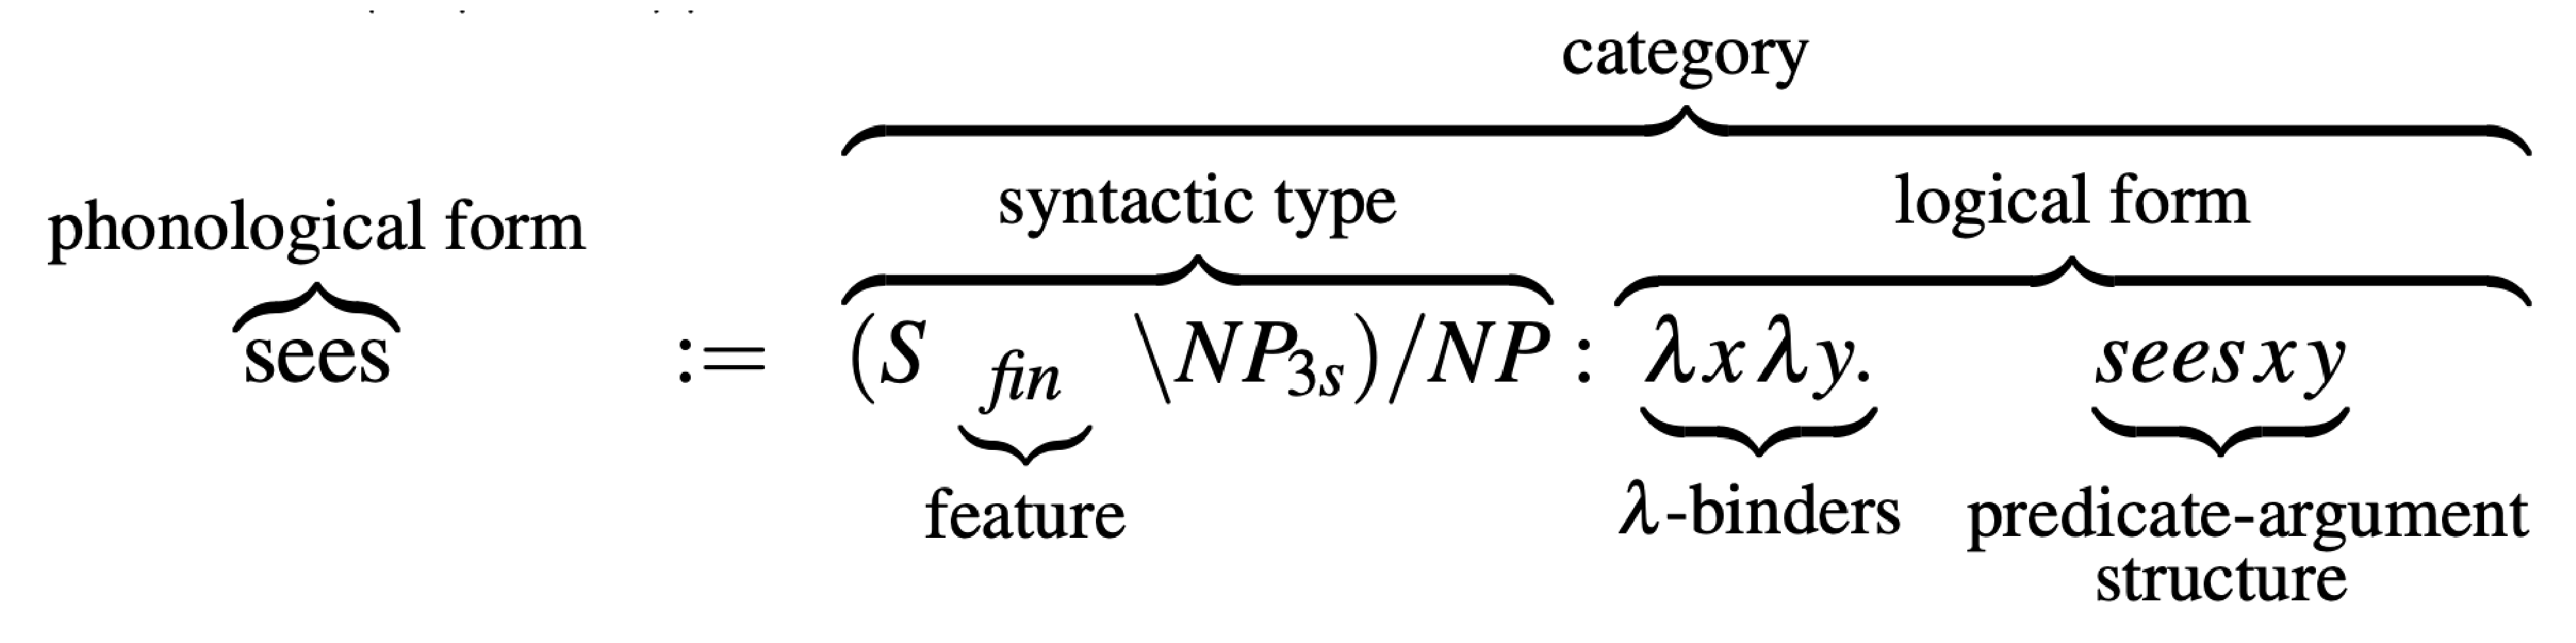
\includegraphics[width=0.8\textwidth]{ccg_forms.eps}
\caption{\cite{steedman_combinatory_nodate} Diagram explaining the mains terms used in CCG}
\label{fig:ccg_forms}
\end{figure}

In the \textit{syntactic type} of a word, the forward slash / indicates forward application to combine terms, while \textbackslash \ indicates backward combination. If there is no slash, then the expression can be thought of as a clause, and it can combine with any rule.

\begin{itemize}[nolistsep]
\item $X/Y:f \quad Y:a \implies X:fa$\quad($>$)
\item $Y:a \quad X\backslash Y:f \implies X:fa$\quad($<$)
\end{itemize}

\mbox{}

There also exists a \textit{morphological slash} \textbackslash\textbackslash, which restricts application to lexical verbs, ruling out auxiliary verbs (whose role is purely grammatically, hence they do not play any part in providing information). The \textit{morphological slash} can be used when dealing with reflexive pronouns such as ``themselves". Furthermore, combining rules directly correlates to obtaining a simpler \textit{logical form} with fewer bound variables, as can be seen in Figure \ref{fig:ccg_derivations}.

\begin{figure}[H]
\centering
\begin{subfigure}{0.3\textwidth}
\centering
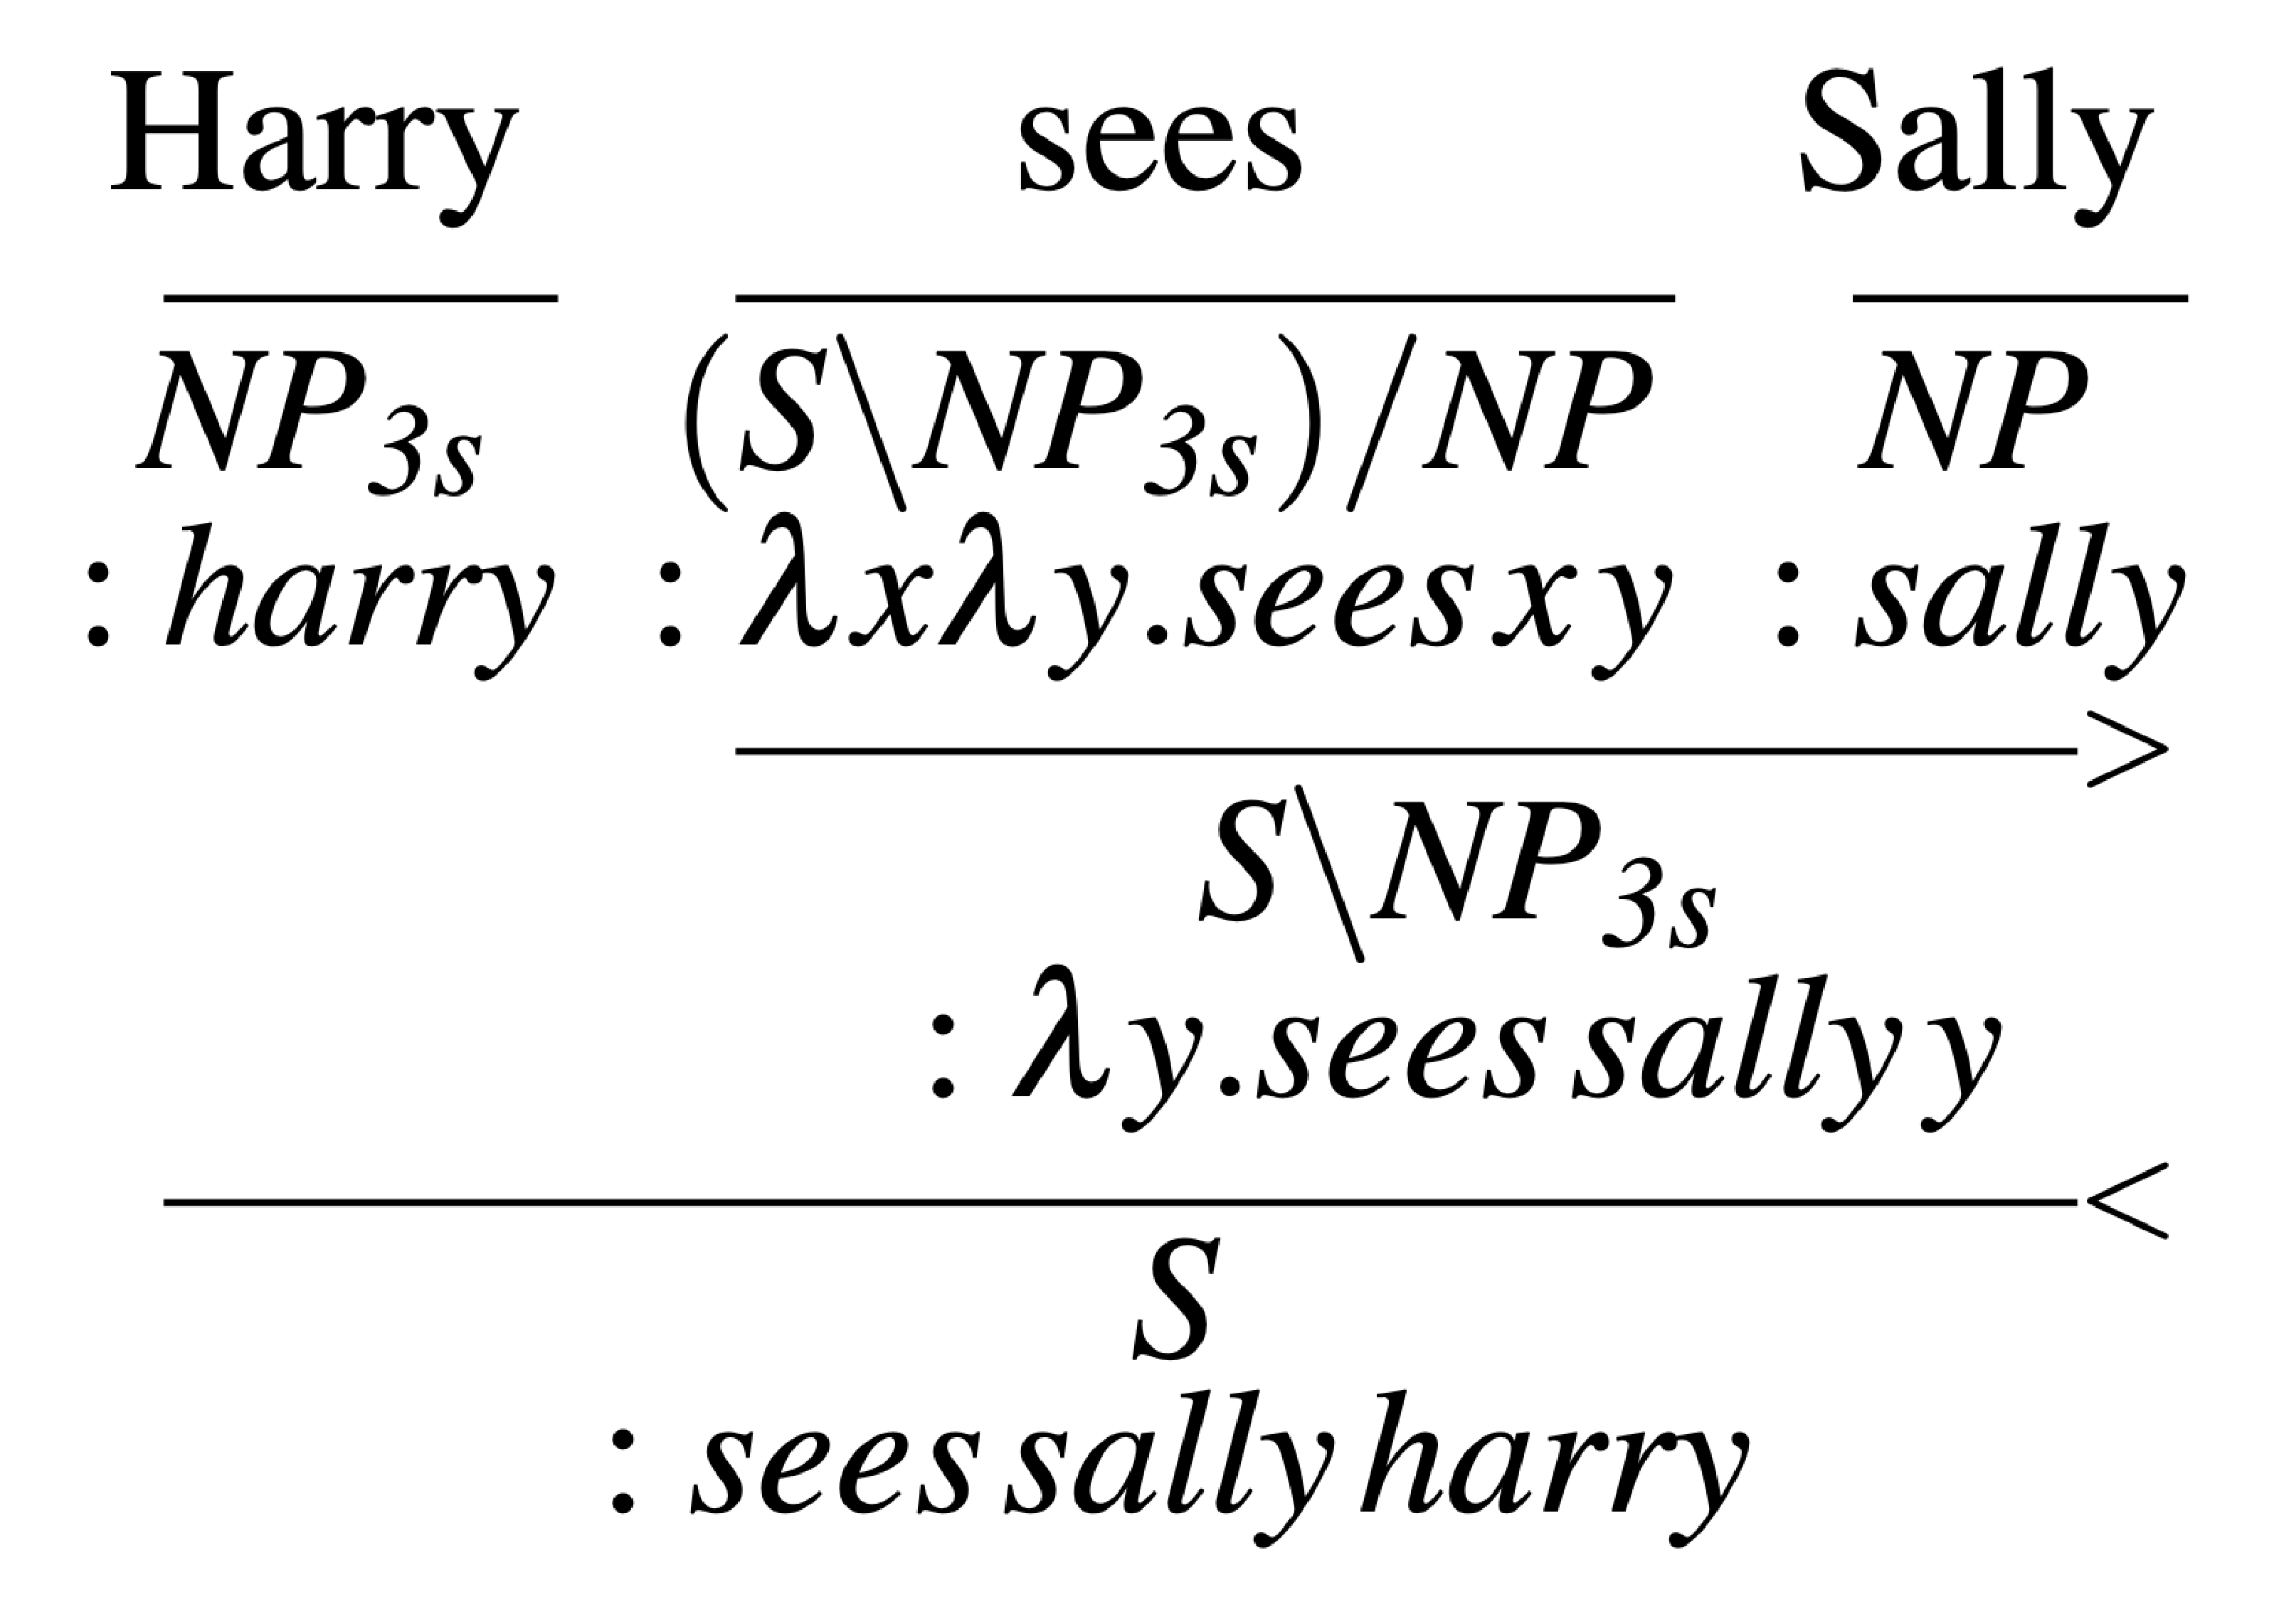
\includegraphics[width=\textwidth]{ccg_basic_derivation.eps}
\caption{\cite{steedman_combinatory_nodate} Basic clause}
\end{subfigure}
\begin{subfigure}{0.6\textwidth}
\centering
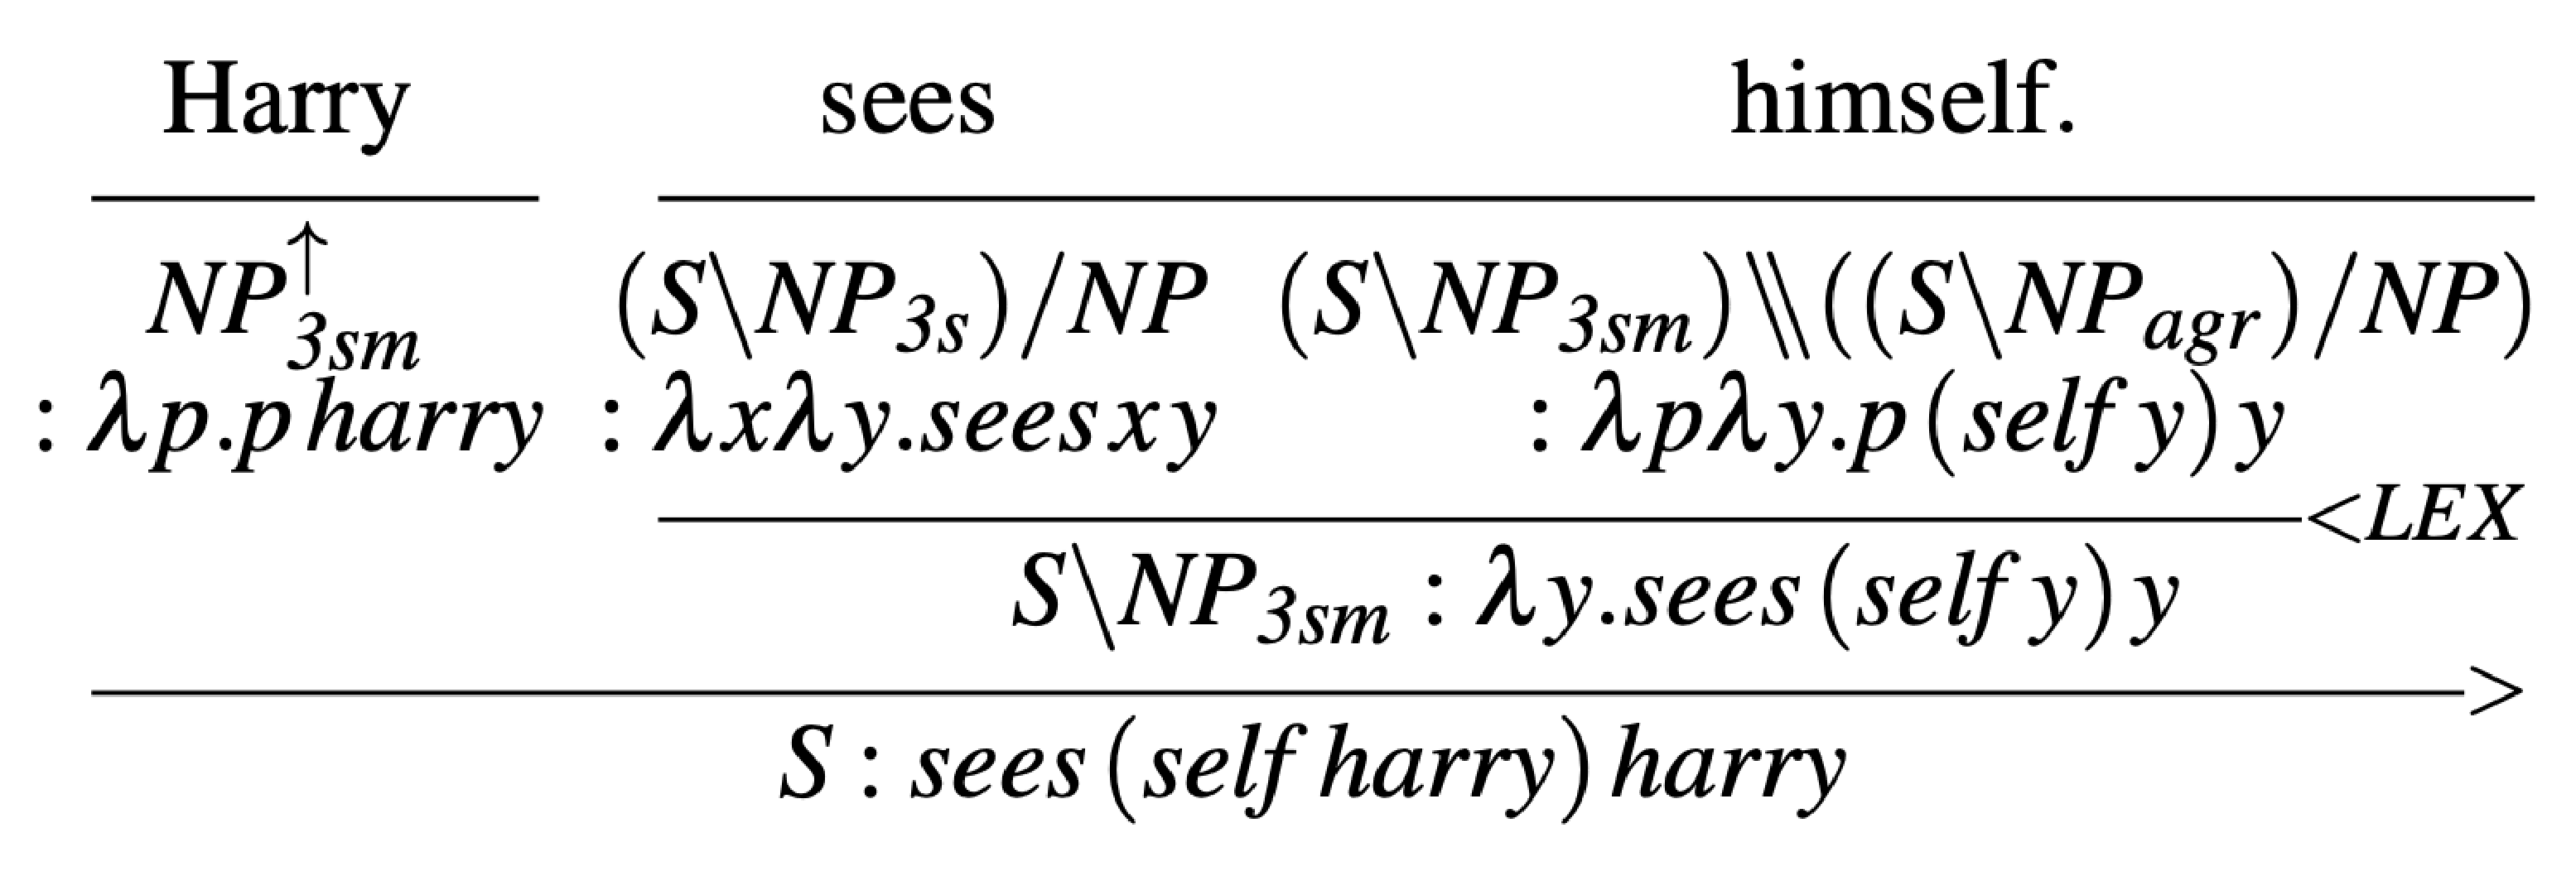
\includegraphics[width=\textwidth]{ccg_reflexive_derivation.eps}
\caption{\cite{steedman_combinatory_nodate} Reflexive transitive clause}
\end{subfigure}
\caption{Examples of derivations in CCG}
\label{fig:ccg_derivations}
\end{figure}

There exist more advanced syntactic rules in CCG, which we shall not go into detail about for the purposes of brevity. However with the basic rules that we explained, you can easily see how this parsing mechanism could be an efficient way to get to the underlying semantics of a sentence. Although the \textit{syntactic type} may seem complicated, it would allows us to get a very precise understanding of English grammar, as well as obtain a simple and consistent \textit{logical form} at the end.

\section{Existing Approaches}

\subsection{MCBA+GA And LSA+TRM}

In a paper by Yeh et al. \cite{yeh_text_2005}, two different methods are put forward for text summarization. The first is the modified corpus-based approach (MCBA), which uses a score function as well as the \textit{genetic algorithm}, while the second (LSA+TRM) utilizes \textit{latent semantic analysis} (LSA) with the aid of a \textit{text relationship map} (TSA).

\mbox{}

In order to understand MCBA, we must first mention corpus-based approaches, which rely on machine learning applied to a corpus of texts and their (known) summaries. In the \textit{training phase} important features (such as sentence length, position of a sentence in a paragraph, uppercase word...) are extracted from the \textit{training corpus} and used to generate rules. In the \textit{test phase} the learned rules are applied on the \textit{training corpus} to generate corresponding summaries. Most approaches rely on computing a weight for each unit of text, this is based on a combination of a unit's features.

The MCBA builds on the basic corpus-based approach (CBA) by ranking sentence positions and using the genetic algorithm (GA) to train the score function. In the first case, the idea is that the important sentences of a paragraph are likely to have the same position in different texts, such as the first sentence (introduction) and the last one (summary). Depending on a sentence's position, a \textit{rank} (from $1$ to some $R$) is assigned, and used to compute a score for this feature. The paper also discusses other features, whose corresponding scores, along with the aforementioned \textit{rank}, are used to compute a weighted sum of all scores. Only the highest scoring sentences are retained in order to form the summary.

Moreover, the \textit{genetic algorithm} (GA) is used to obtain suitable weights, where a \textit{chromosome} is defined by a set of values for all the features weights. Using the notions of \textit{precision} (proportion of predicted positive cases that are correctly real positives) and \textit{recall} (proportion of real positive cases that are correctly predicted positive) \cite{powers_evaluation_2011}, a so-called \textit{F-score} is computed to define the fitness for each chromosome. By combing two \textit{chromosomes} to generate children, where the fittest parents are most likely to mate, we end up (after some number of generations) with a set of feature weights suitable for the corpus in question.

\mbox{}

On the other hand, the LSA+TRM approach comprises four major steps: \textit{preprocessing} (1), \textit{semantic model analysis} (2), \textit{text relationship map construction} (3) and \textit{sentence selection} (4).

In step (1), sentences are decomposed according to their punctuation, as well as divided into keywords.

In step (2), a \textit{word-by-sentence matrix} is computed on the scale of the entire document (or corpus). This  gets factorized and reduced to leave out words which do not occur often, then turned into a \textit{semantic matrix} linking words to their according relevance with each sentence.

In step (3), the \textit{semantic matrix} is converted to a \textit{text relationship map}. A \textit{text relationship map} is a graph comprised of nodes, each one represents a sentence or paragraph. A link exists between any two which have high semantic similarity, and the idea is that nodes with many links are likely to cover the main topics of the text.

Finally, step (4) uses the \textit{text relationship map} to pick out the most important sentences for the summary. Figure \ref{fig:lsa_trm_diagrams} may help you visualize how this works.

\begin{figure}[H]
\begin{subfigure}{0.5\textwidth}
\includegraphics[width=\textwidth]{lsa_trm_diagram.eps}
\caption{\cite{yeh_text_2005} Overall process}
\end{subfigure}
\begin{subfigure}{0.5\textwidth}
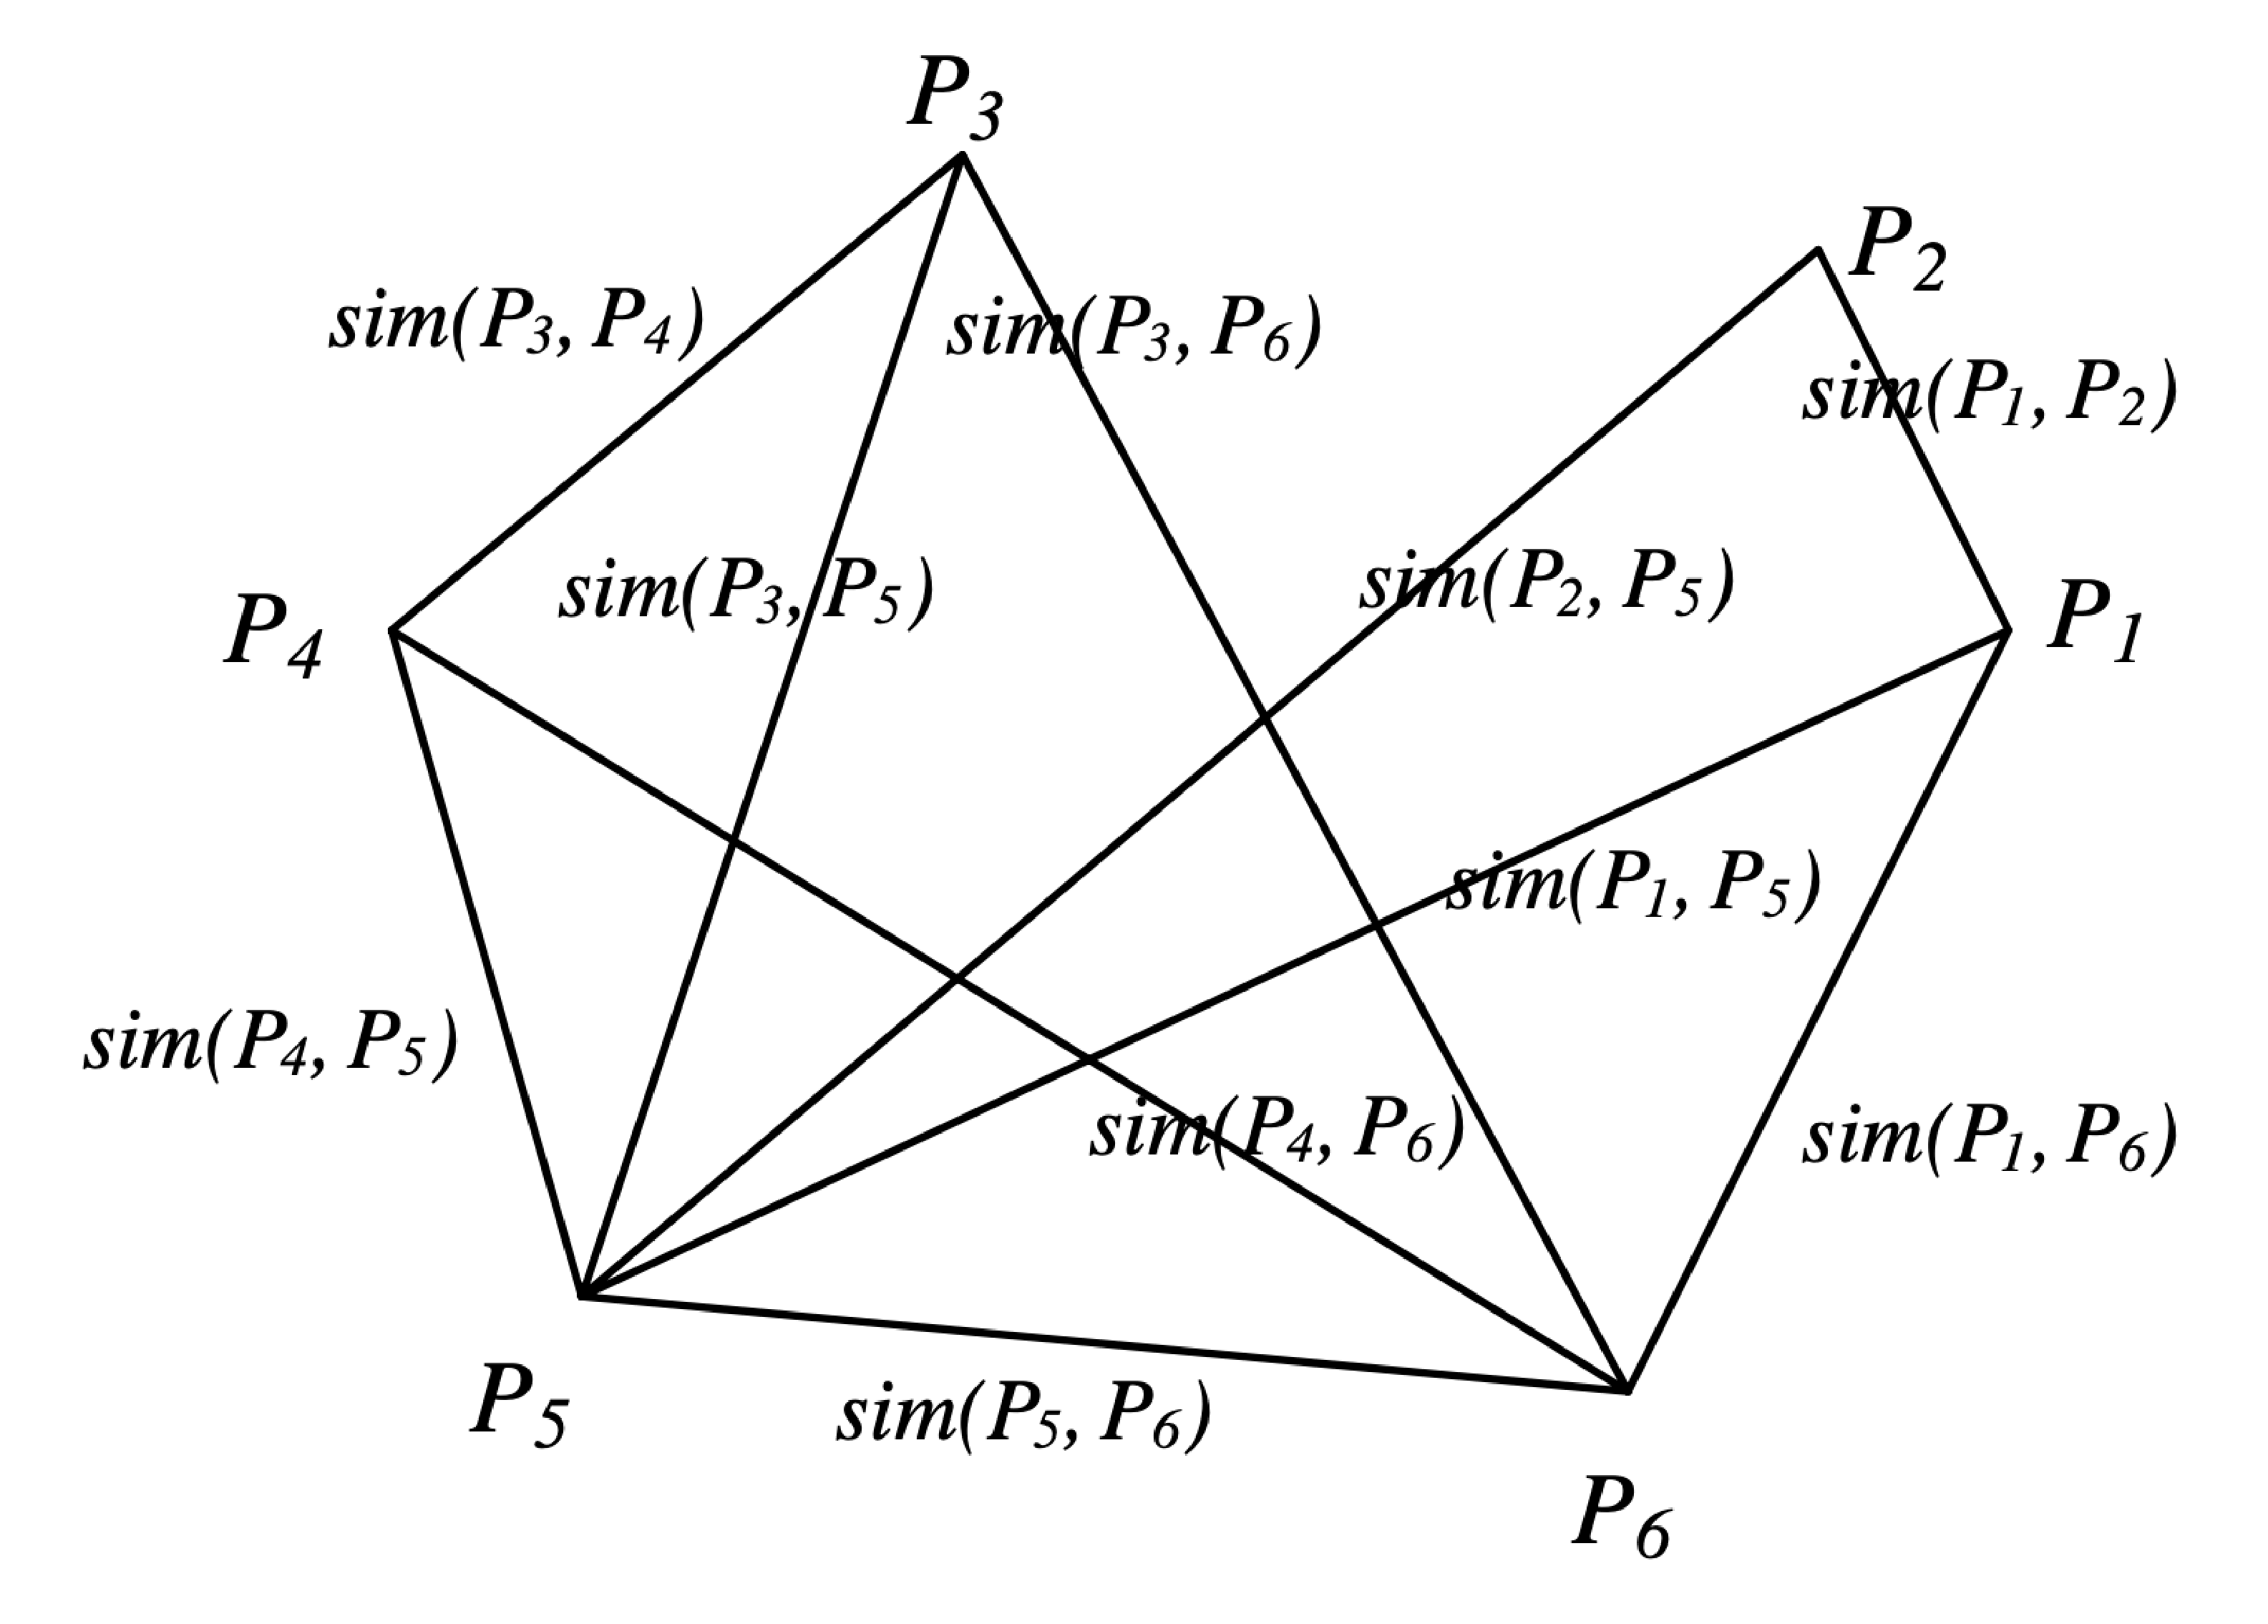
\includegraphics[width=\textwidth]{text_relationship_map_diagram.eps}
\caption{\cite{yeh_text_2005} Example of a text relationship map}
\end{subfigure}
\caption{LSA+TRM approach, diagrammatically}
\label{fig:lsa_trm_diagrams}
\end{figure}

\textit{Compression rate} (CR) is a proportion describing the size of the summary with respect to the size of the original text.

After evaluating both approaches on a news article corpus, it was found that MCBA outperforms the basic CBA by around 3\%, confirming the hypothesis that the position of a sentence plays a role in its importance. Furthermore, MCBA+GA performs around 10\% better than MCBA.% However, the difference in genre between the \textit{training corpus} and \textit{test corpus} has an influence on the performance of GA.

Concerning LSA+TRM, it was found that on a per-document level this approach outperformed simply using TRM with the sentence keywords rather than LSA by almost 30\%. It was thus concluded that LSA helps get a better semantic understanding of a text.% On a corpus-level, this performance improvement is only around 20\%.

Comparing the two approaches highlighted in the paper, it is mentioned that performance is similar, although LSA+TRM is easier to implement than MCBA in single-document level as it requires no preprocessing, and in some optimal cases performs up to 20\% better. Although the former approach is more computationally expensive, it is more adept at understanding the semantics of a text because it does not rely on the genre of the corpus that was used for training. In both cases though, performance improves as CR increases.

\mbox{}

As our solution will rely on ASG, no machine learning will be needed. However, the first approach is still interesting in the sense that it uses a certain number of important features to identify the important sentences of a passage. In our approach, we may want to use some of these metrics to construct the summary.

From the second approach, the main takeaways are the storage mechanisms in use such as the \textit{semantic matrix} and \textit{text relationship map}. In our system we may also want to use the idea that sentences or \textit{chunks} which are semantically similar to many others in the \textit{text relationship map} are likely to cover the main topics of a passage.

Finally, we notice that the approach based on machine learning (MCBA) gives summaries of inferior quality in general, confirming that the use of ASG is a good choice. In addition, it was found that the longer the summary (higher CR), the more accurate it is, so we must be particularly careful when generating one to two sentence summaries.

\subsection{Lexical Chains}

In a paper about \textit{lexical chains} \cite{barzilay_using_1997}, the authors describe a method which relies on semantic links between words. The idea is that we establish chains of related words, in order to learn what a text is about.

In order to create such a chain, the algorithm begins by choosing a set of \textit{candidate words} for the chain. These \textit{candidate words} are either nouns, or \textit{noun compounds} (such as ``analog clock"). Starting from the first word, the task is to find the next related word which has a similar meaning (a dictionary is used here). If the word has multiple senses, then the chain gets split into multiple interpretations; this process continues until we have analysed all \textit{candidate words}.  For instance, the word ``person" can be interpreted as meaning a human being (\underline{interpretation 1}), or as a grammatical term used for pronouns (\underline{interpretation 2}). An example for the below text is shown in Figure \ref{fig:lexical_chain_example}.

\begin{displayquote}
\textbf{Mr.} Kenny is the \textbf{person} that invented an anesthetic \textbf{machine} which uses \textbf{micro-computers} to control the rate at which an anesthetic is pumped into the blood. Such \textbf{machines} are nothing new. But his \textbf{device} uses two \textbf{micro-computers} to achieve much closer monitoring of the \textbf{pump} feeding the anesthetic into the patient. \cite{barzilay_using_1997}
\end{displayquote}

Furthermore, \textit{lexical chains} are attributed a \textit{strength}, which is based on three criteria: repetition (of the same word), density (the concentration of chain members in a given portion of the text) and length (of the chain). For instance, the \textit{lexical chain} beginning with the word ``machine" shown in Figure \ref{fig:lexical_chain_example} (\underline{interpretation 1}) has considerable repetition, moderate density, and is quite long (it spans almost the entire text).

Based on this indicator, interpretations of a \textit{lexical chain} with higher \textit{strength} will be preferred. (In reality this is a bit more complex, but we will omit the details for simplicity.)

\begin{figure}[H]
\centering
\begin{subfigure}{0.45\textwidth}
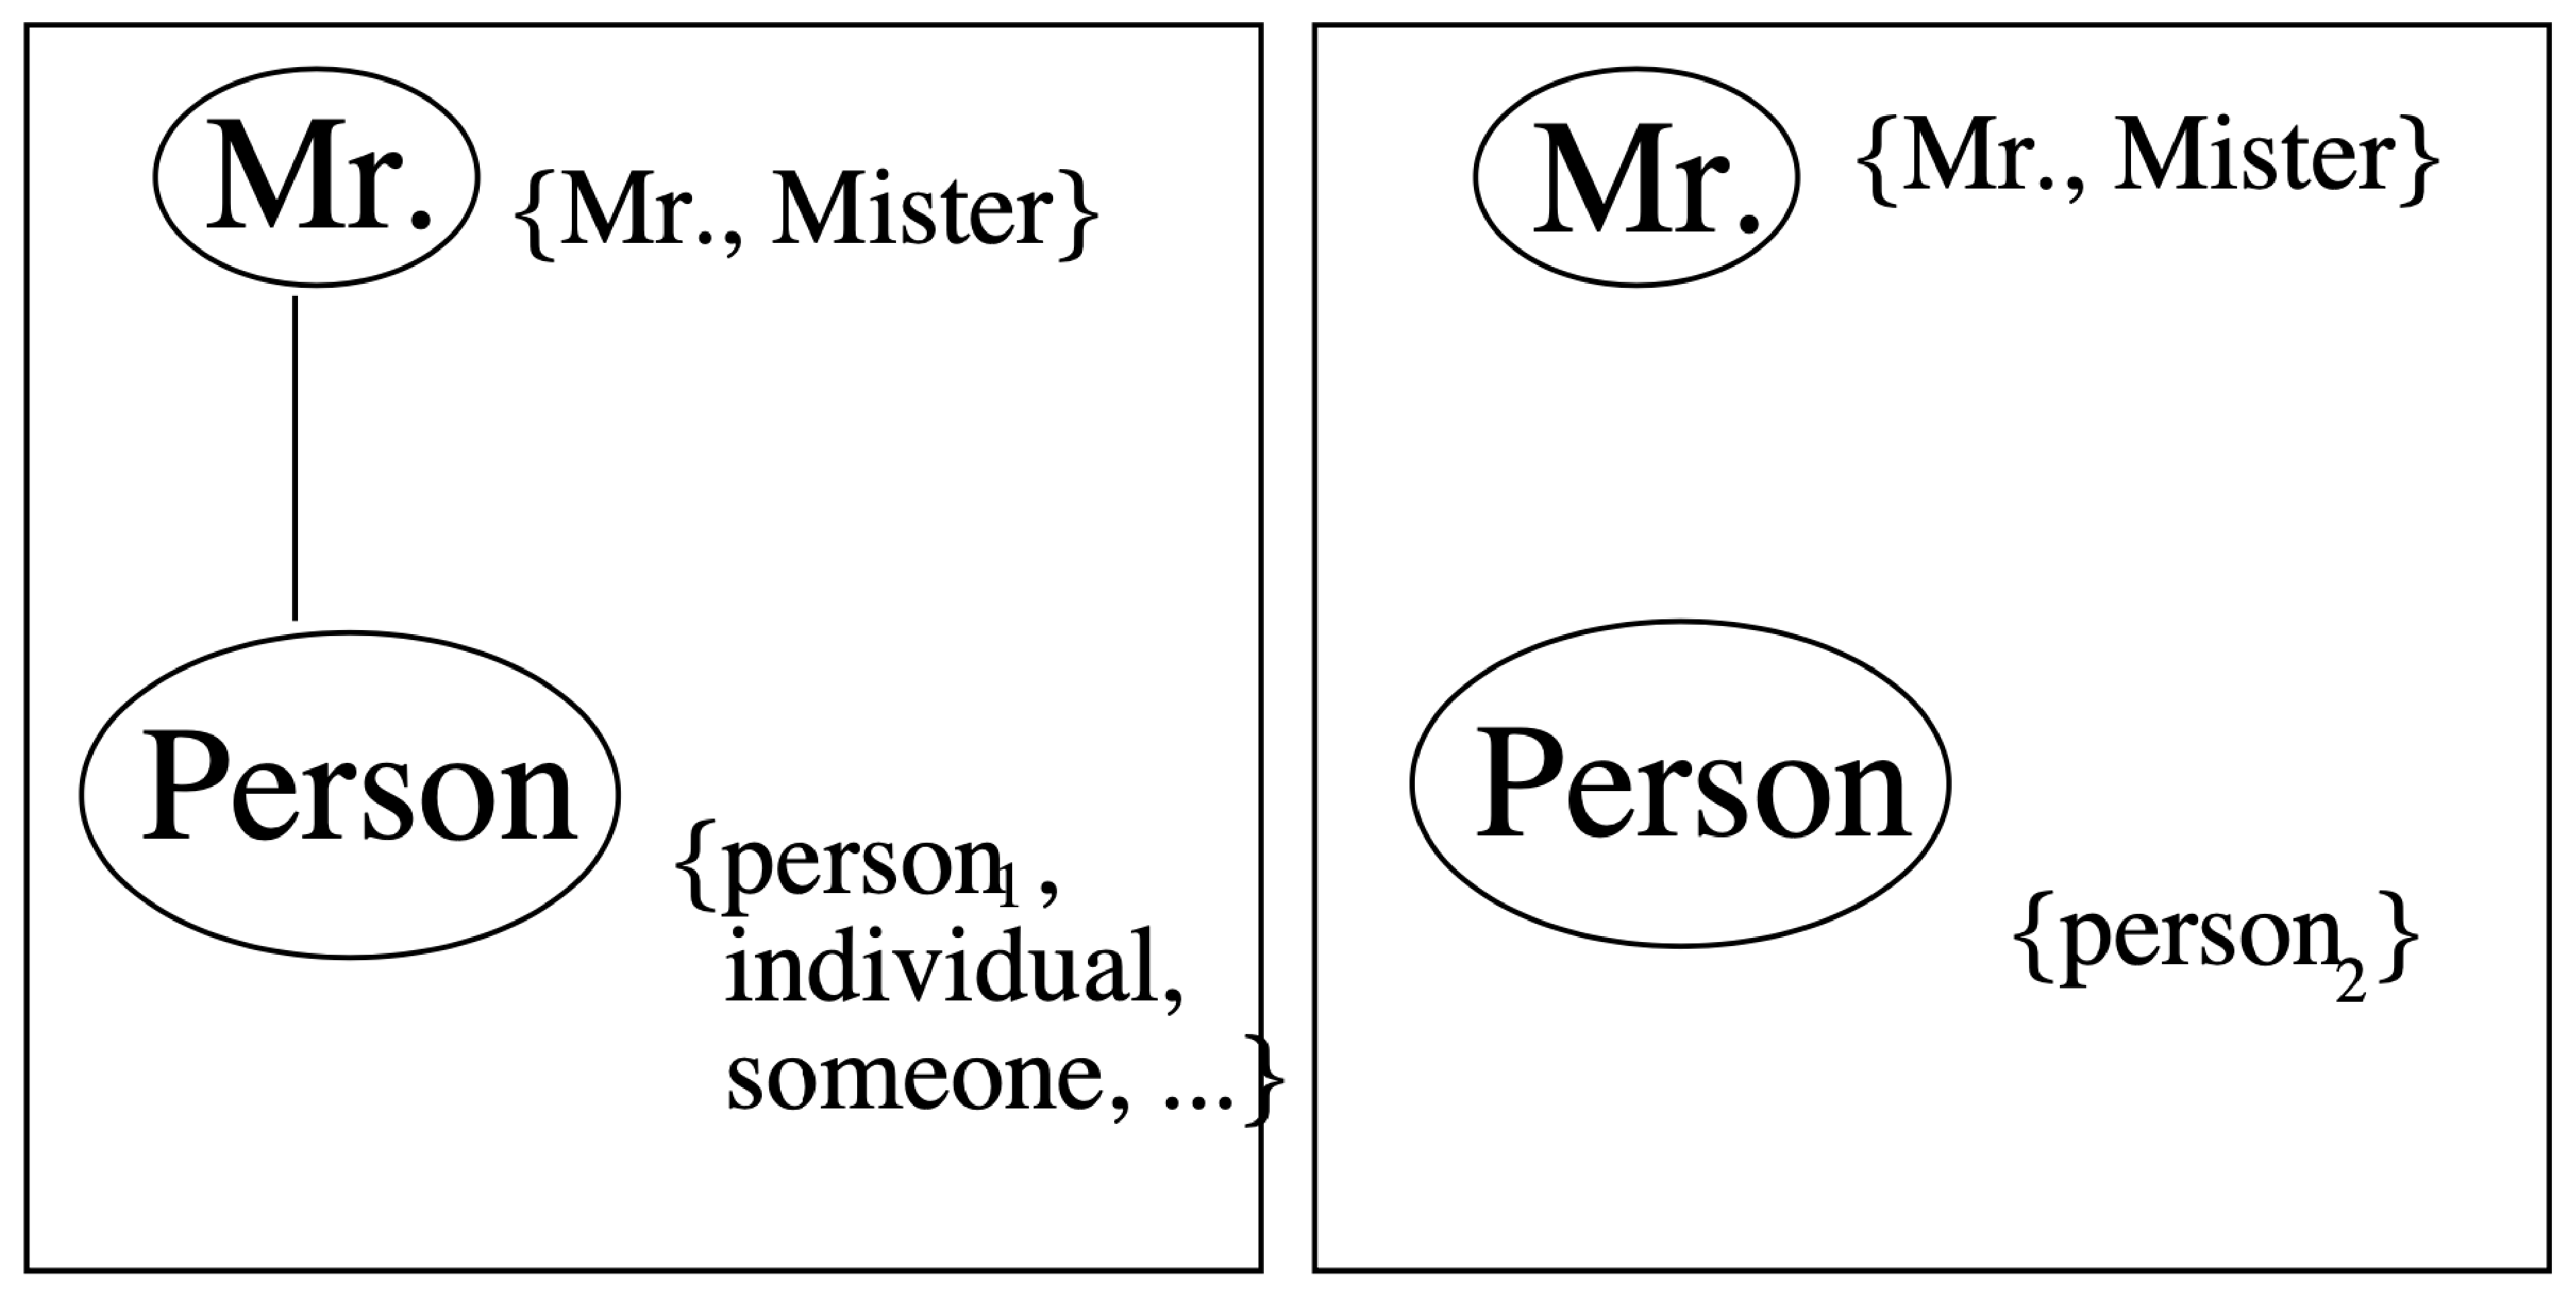
\includegraphics[width=\textwidth]{lexical_chains_step_1.eps}
\caption{Step 1, interpretations 1 and 2}
\end{subfigure}
\begin{subfigure}{0.35\textwidth}
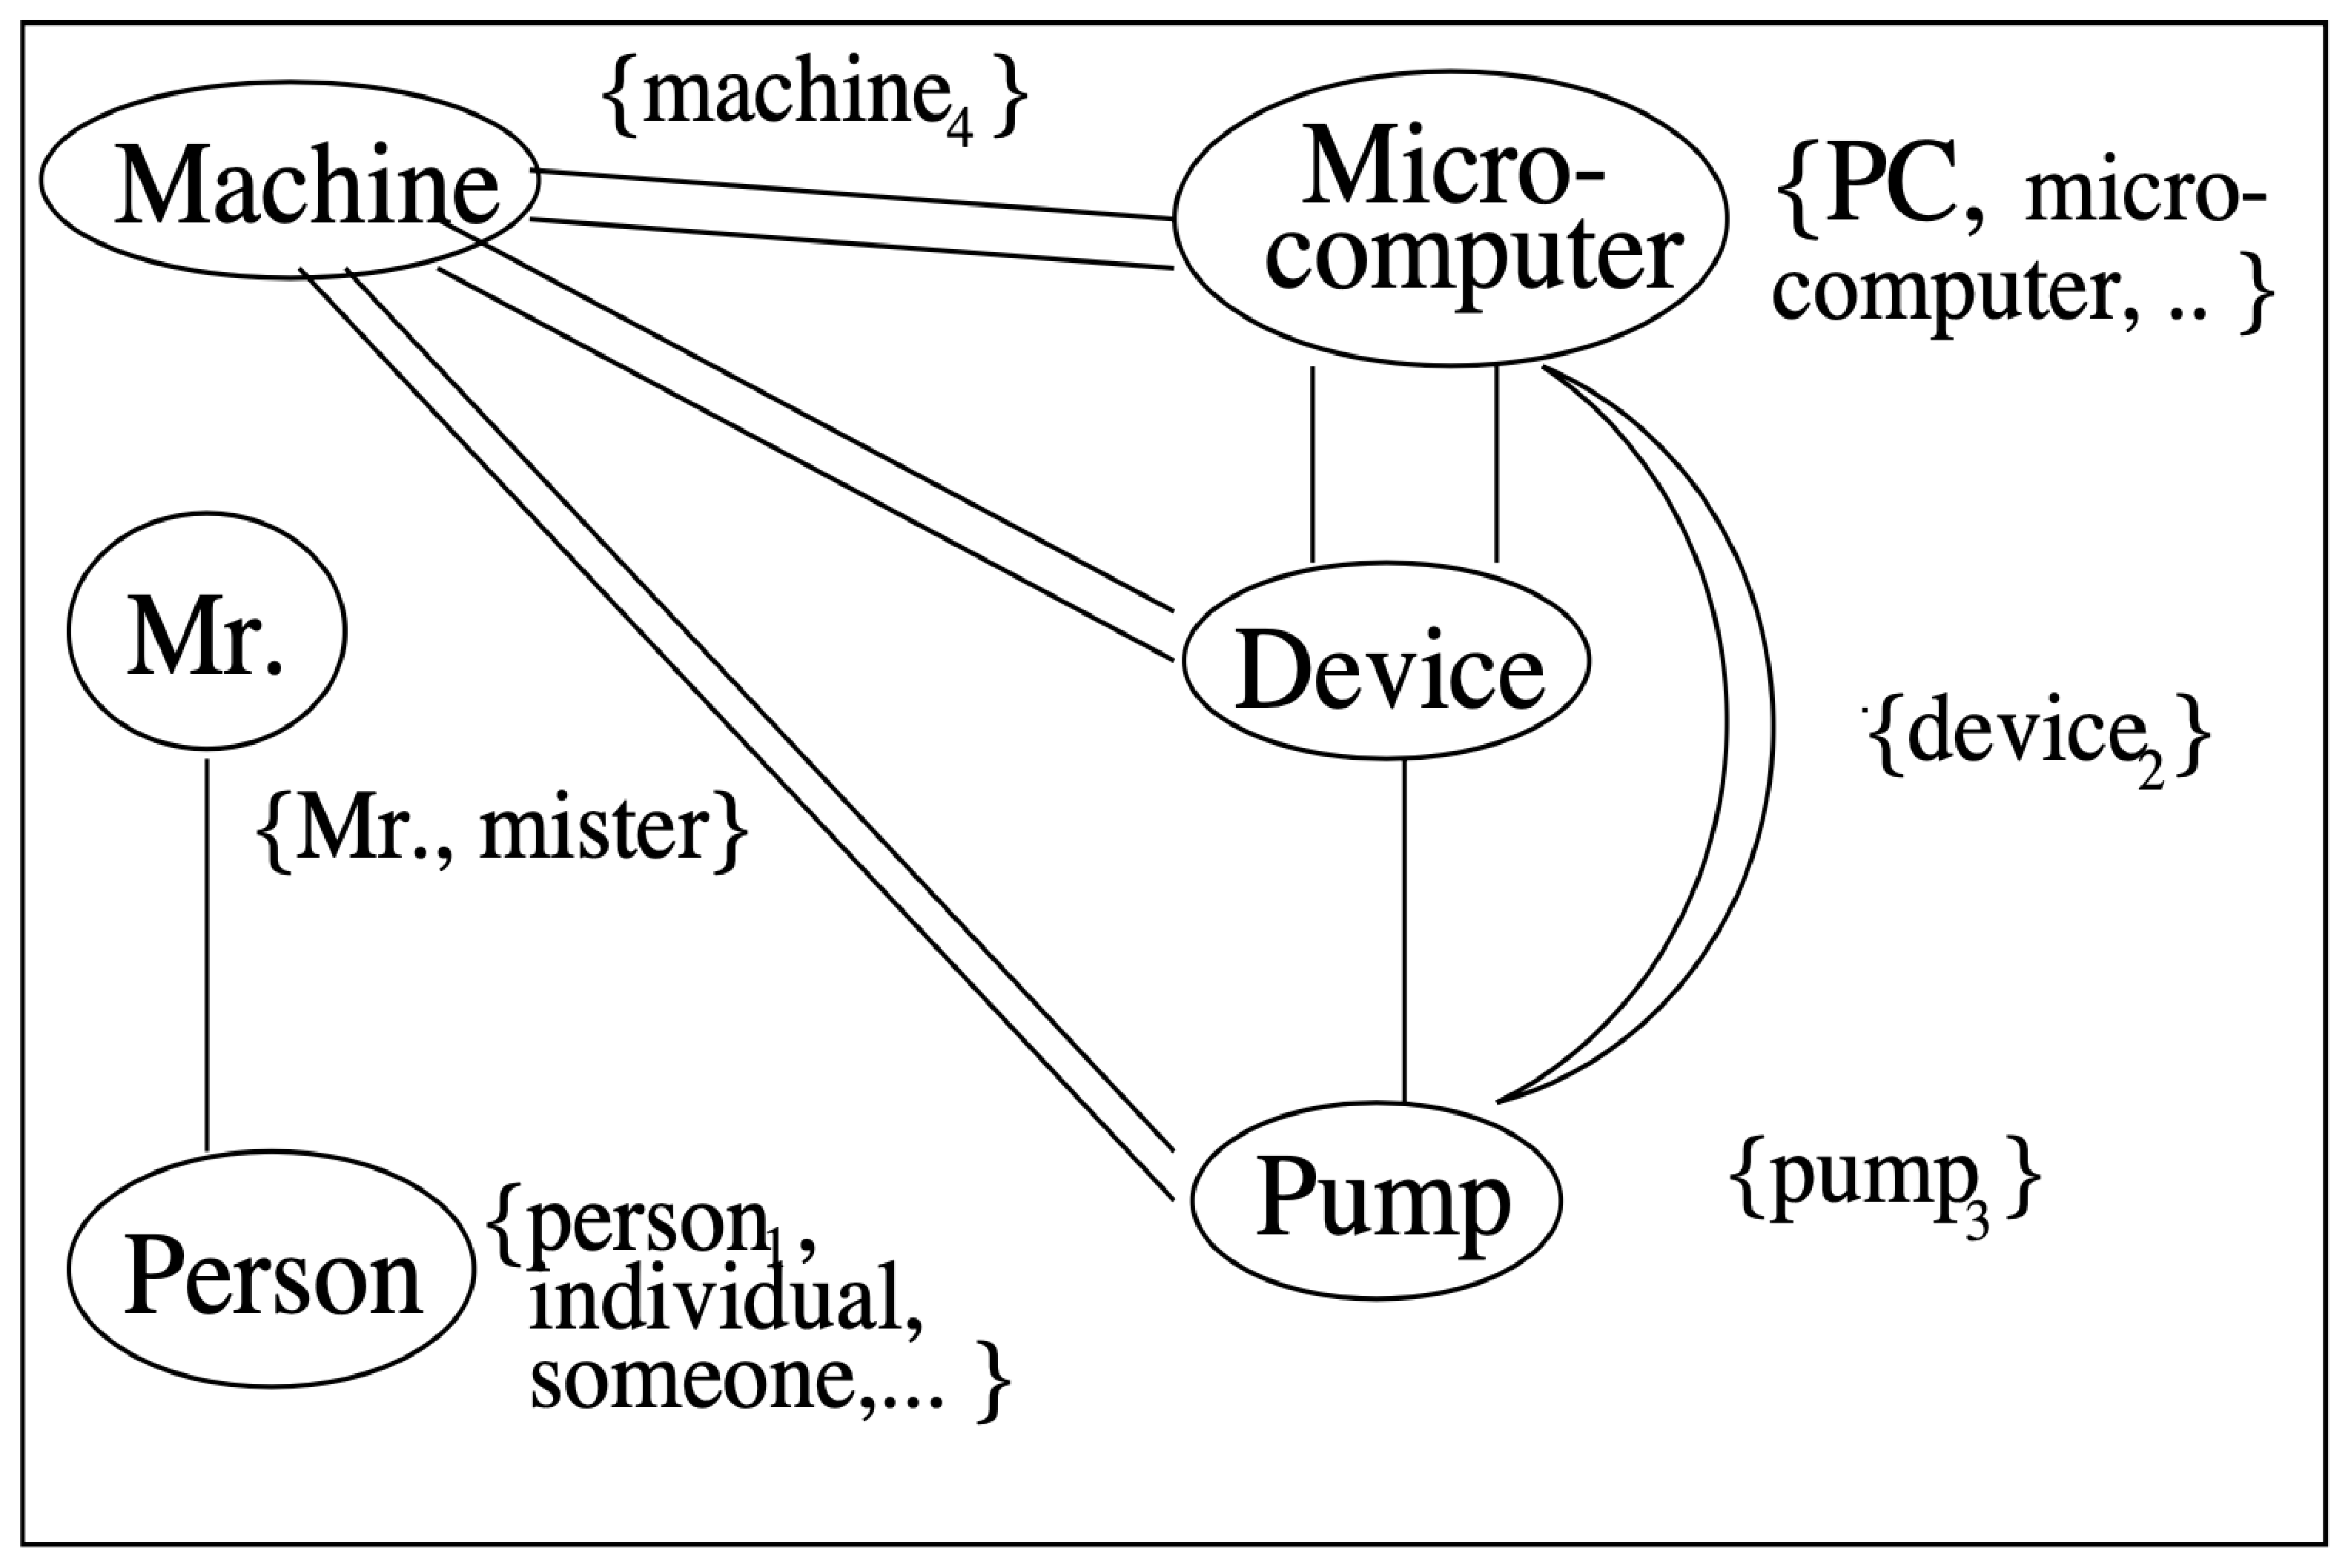
\includegraphics[width=\textwidth]{lexical_chains_step_3.eps}
\caption{Step 3, interpretation 1}
\end{subfigure}
\caption{\cite{barzilay_using_1997} Example of a \textit{lexical chain} and its interpretations}
\label{fig:lexical_chain_example}
\end{figure}

In order to construct the summary, a single ``important" sentence is extracted from the original text. To this end, they use a heuristic which is based on the fact that an important topic will discussed across the entire passage. Once a \textit{lexical chain} has been chosen according to this metric (i.e., one that is well distributed across the text), the output of the algorithm is the sentence which has the highest number of words from the selected \textit{lexical chain}.

\mbox{}

Although the proposed solution is very interesting in that it tries to link important words, it does not do anything whatsoever to learn any of the actions which are described in a passage. This means it has no knowledge of chronology (problematic when we have an action causing a change of state, such as a someone acquiring a good), nor does it try to link subjects with objects or verbs (for instance in the phrase ``Mary has a pencil", it does not link Mary to the pencil).

Furthermore, the algorithm outputs a singe unchanged sentence from the original text; this is suboptimal when equally important information is conveyed across multiple sentences. In a solution to the problem of text summarization, we would hope that important facts or actions are given as a summary. For the approach discussed here, this would mean picking out \textit{chunks} of text from the original passage, and combining them in a suitable manner.

\section{Approach Categories}

\subsection{Statistical}

In the statistical approach, the methodology is to use probabilities in order to generate a summary that is both grammatically correct and conveys the important details of a text.

\mbox{}

The authors of the paper \cite{knight_statistics-based_2000} envision what they call a \textit{noisy-channel model}, which at the time of writing was limited to single sentence summarization. For the  model, assume that there was at some point a (shorter) summary string $s$ for the (longer) string $t$ to summarize, from which optional words were removed. The idea is that optional details were added to produce $t$, and we want to know with what probability $s$ contained this information given $t$. At this stage, there a three problems to solve:
\begin{enumerate}[noitemsep]
\item To obtain the \textit{source model}, we must assign a probability $P(s)$ to every string $s$, which tells us how likely it is that this is the summary. If we assign a lower $P(s)$ to less grammatically correct strings, then it helps ensure that our final summary is well-formed.
\item To obtain the \textit{channel model}, we now assign the probabilities $P(t \vert s)$ to every pair $\langle s, t \rangle$. This contributes to preserving important information, as we take into account the differences between $s$ and $t$ when computing the corresponding probability. In this case, we may want to assign a very low $P(t \vert s)$ when $s$ omits an important verb or negation (these are not optional to get the correct meaning), while this can sometimes be much higher if the only difference is the word ``that".
\item For a given string $t$ the goal is now to maximize $P(s \vert t)$ which, because of \href{https://www.investopedia.com/terms/b/bayes-theorem.asp}{Bayes' theorem}, is equivalent to maximizing $P(s) \cdot P(t \vert s)$.
\end{enumerate}

In practice, the implementation discussed in the paper uses \textit{parse trees} rather than whole strings. Also, they use machine learning techniques in order to train their summarizer.

To this end, they created what was referred to in the paper as a \textit{shared-forest} structure, allowing them to represent all compressions given an original text $t$; an example is shown in Figure \ref{fig:statistics_example}. Their system picks out high-scoring trees from the forest, and based on this score we can choose the best compression $s$ for $t$ (i.e., the summary $s$ which has the highest $P(s) \cdot P(t \vert s)$).

If the user wants a shorter or longer summary, the system can simply return the highest-scoring tree for a given length. In reality though their solution is a bit more complex, but the important points of the approach are here.

\begin{figure}[H]
\begin{subfigure}{0.3\textwidth}
\quad \\
\quad \\
\phantom{\qquad}A $\rightarrow$ B C D \\
\phantom{\qquad}A $\rightarrow$ B C \\
\phantom{\qquad}A $\rightarrow$ C D \\
\phantom{\qquad}A $\rightarrow$ B D \\
\phantom{\qquad}A $\rightarrow$ B \\
\phantom{\qquad}D $\rightarrow$ E F \\
\phantom{\qquad}D $\rightarrow$ E \\
\phantom{\qquad}D $\rightarrow$ F \\
\caption{\textit{Shared-forest} structure}
\end{subfigure}
\begin{subfigure}{0.4\textwidth}
\centering
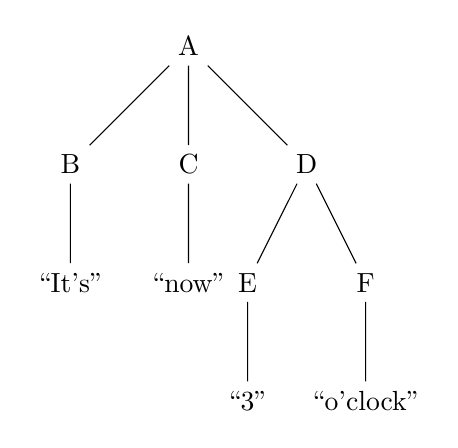
\begin{tikzpicture}
\node {A}
  child {node {B}
    child {node {``It's"}}}
  child {node {C}
    child {node {``now"}}}
  child {node {D}
    child {node {E}
      child {node {``3"}}}
    child {node {F}
      child {node {``o'clock"}}}};
\end{tikzpicture}
\caption{\textit{Parse tree} for $t$}
\end{subfigure}
\begin{subfigure}{0.25\textwidth}
\centering
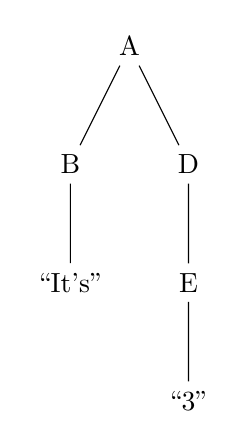
\begin{tikzpicture}
\node {A}
  child {node {B}
    child {node {``It's"}}}
  child {node {D}
    child {node {E}
      child {node {``3"}}}};
\end{tikzpicture}
\caption{\textit{Parse tree} for $s$}
\end{subfigure}
\caption{Example of an original text $t$ and possible summarization $s$}
\label{fig:statistics_example}
\end{figure}

In their testing it was found that their algorithm has a conservative nature, promoting correctness over brevity, which sometimes has the consequence of not trimming any words away. Therefore, this implementation is highly unsuitable for our purposes, but we shall nonetheless keep in mind the notion of the \textit{shared-forest} structure, as well as the use of Bayesian probability theory.

%In the decision-based model, they apply a sequence of shift-reduce-drop operations on the original sentence's parse tree \textit{t} in order to obtain the compressed sentence \textit{s} in the form of a stack. Starting from an empty stack, they are able to get a summary that can have a different ordering of words, which is not possible using the \textit{noisy-channel model}.

%After training these models using a set of newspaper articles with abstracts, they found that both were significantly better than the baseline they were using, although performed worse than humans. When run on a different dataset, they found that the decision-based model produced sentences that were more grammatically correct, however they would often be slightly over-compressed.

\subsection{Frame}

In the frame approach, the idea is that we try and keep track of how the plot in a story progresses, recording each action as well as the links which connect them. From this understanding, we should then have enough information to build an accurate summary.

\mbox{}

In one of the original papers describing this approach \cite{lehnert_1980_nodate}, sentences are decomposed into different \textit{affect states} and \textit{affect links}. An \textit{affect state} can either be a \textit{mental state}, or a \textit{positive} or \textit{negative event} which may cause a change to a \textit{mental state}. \textit{Affect links} are then the transitions that explain the sequence of \textit{affect states}.

We are given the example of John and Mary who both want to buy the same house, but it ends up being sold to Mary. At the start, both characters have the same \textit{mental state} (desire to buy the house). However the \textit{actualization} (a type of \textit{affect link} which denotes realization of an action) of Mary's desire is recognized as a \textit{positive event} for Mary and a \textit{negative event} for John.

By combining sequences of \textit{affect links} (transitions) between \textit{affect states} for different characters in a story, it is easy to see how one can build the narrative of the entire text. Such an example is shown in Figure \ref{fig:frame_example}, where \textit{m} denotes the \textit{motivation affect link} (connecting an action with a \textit{mental state} which it motivates), and \textit{e} denotes the \textit{equivalence affect link} (i.e., when a character has the same \textit{mental state} before and after the transition).

\begin{figure}[H]
\centering
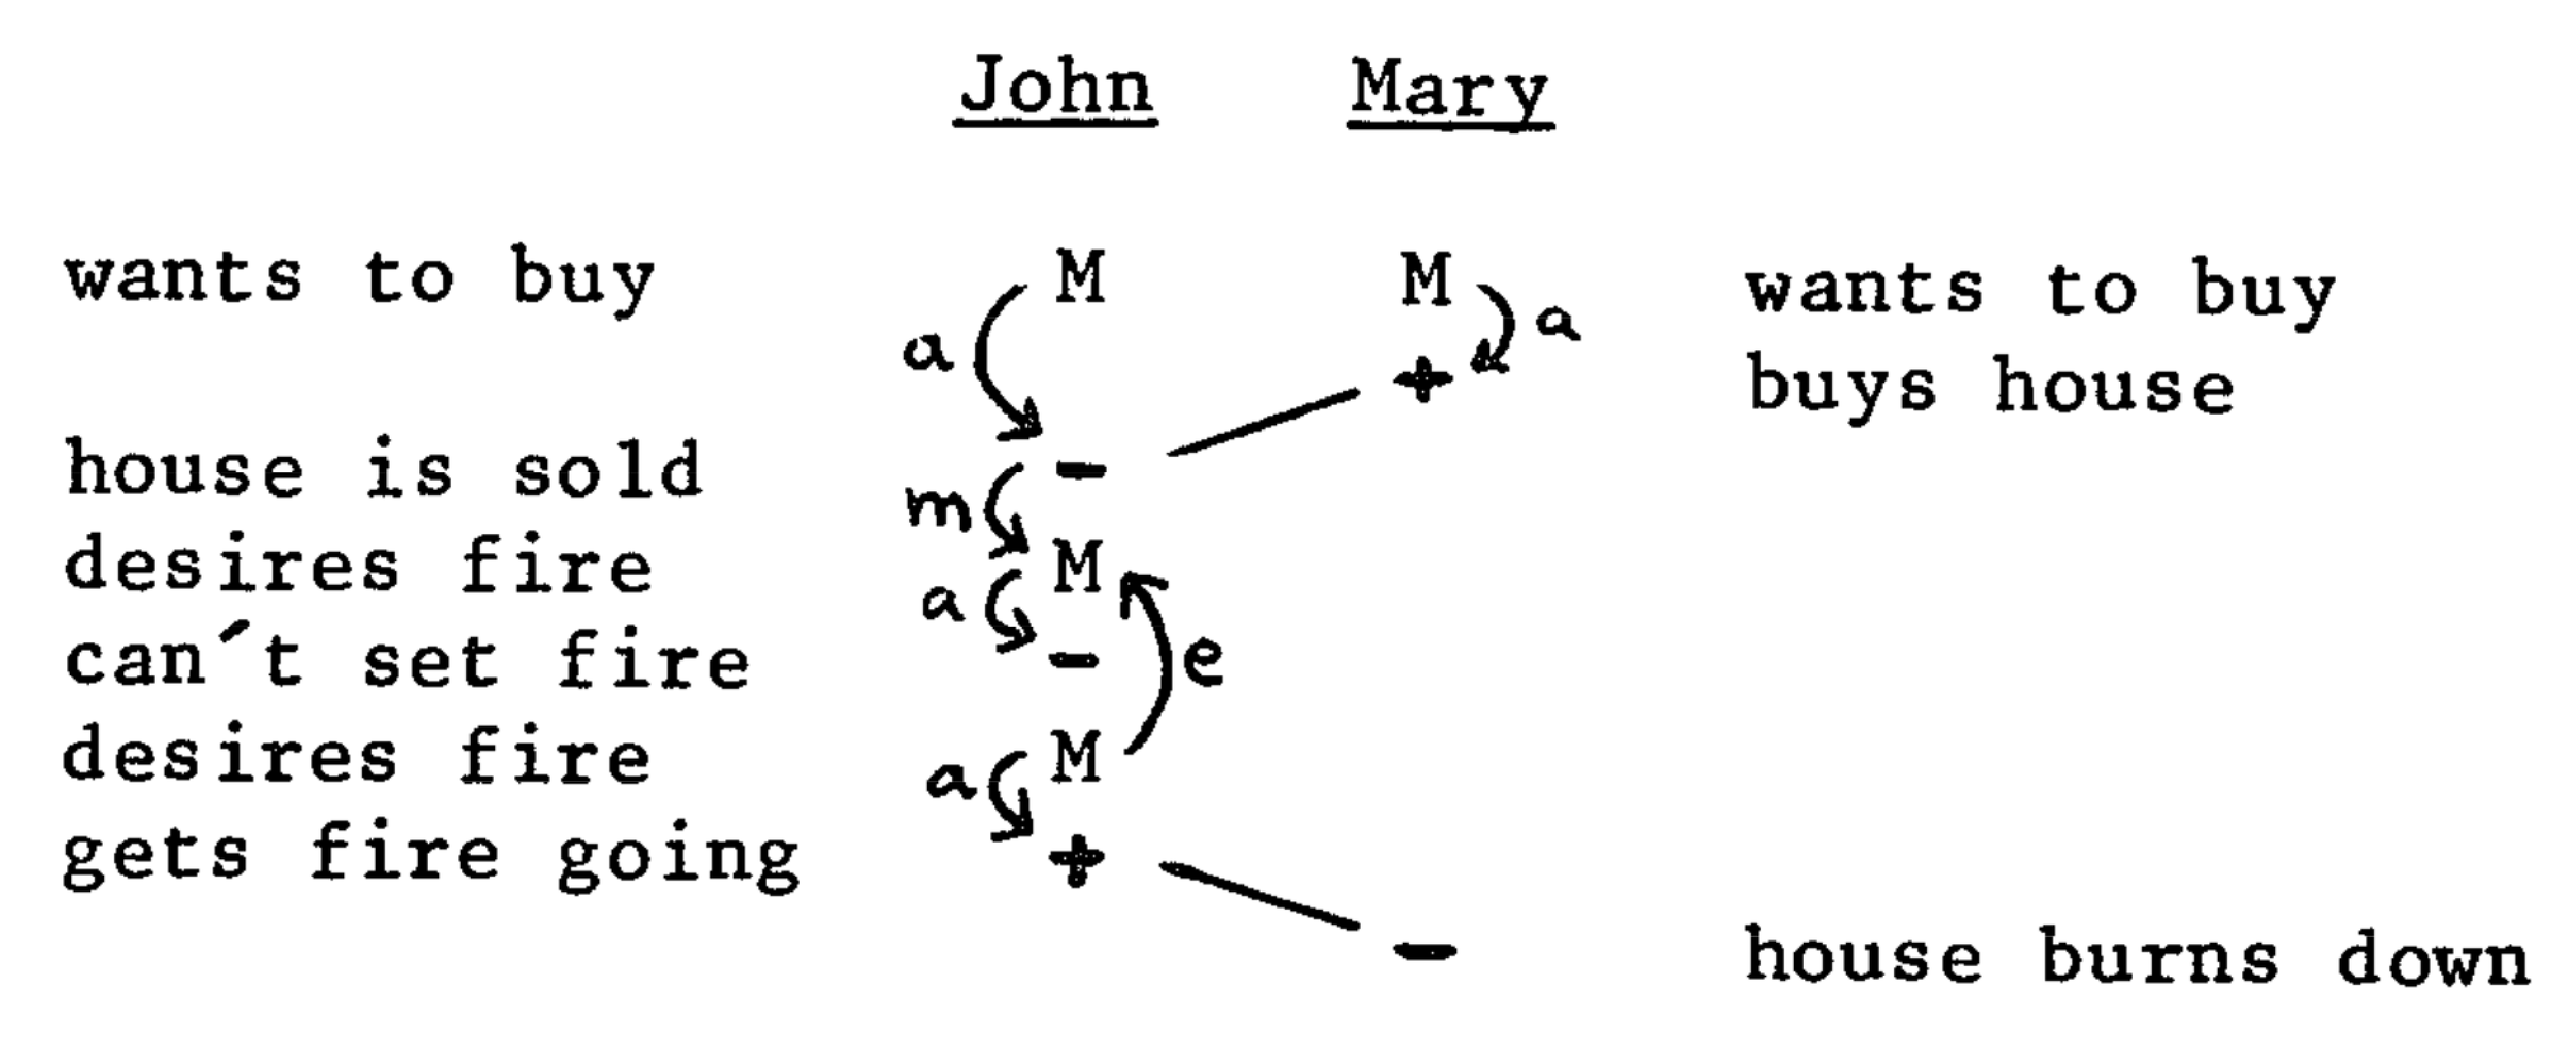
\includegraphics[width=0.7\textwidth]{frame_example.eps}
\caption{Example of a narrative in the frame approach}
\label{fig:frame_example}
\end{figure}

While this approach is interesting from a semantic point of view, it can easily become very complicated when many sentences are involved. In addition, it would not be suitable for purely descriptive texts, involving only continuous actions without any direct link (``It was October. Leaves were falling from the trees.").

\subsection{Symbolic}

In the symbolic approach \cite{clark_combining_nodate}, meaning is expressed through logic, and the representation of a sentence is the combination of the meaning of each of its individual components. CCG, as discussed in Subsection \ref{ssec:ccg}, uses a symbolic approach.

Generally the semantics of a word is captured as a single predicate in logic, and sometimes this is automatically derived from a large dataset such as an online dictionary. In order to obtain the final (sentential) logical form however, parsed sentences (represented for example as a \textit{parse tree}) must first be translated from their original (natural language) syntax. It then becomes possible to combine the meanings of words to obtain sentence fragments, and then combine these to understand the whole sentence. These can be further composed to cover an entire passage. This representation can then be provided to a theorem prover in \textit{first-order logic} (FOL), or directly converted into a logic program (for instance in ASP).

\mbox{}

Besides CCG, another pertinent case study is that of the Montague Grammar \cite{partee_lecture_nodate}. In such a grammar, we have what is called a \textit{syntactic language} and a \textit{semantic language}. The former is similar to POS tags (see Appendix \ref{appendix:pos}), while the latter captures the type of a token (which can either be $e$ for \textit{entity} or $t$ for \textit{truth value}). For instance, the word ``John" has \textit{syntactic category} ProperN and \textit{semantic type} $e$, while for the verb ``walks" these are respectively VP and $e \to t$.

For both of these languages, there exist rules that dictate how we are allowed to compose tokens. In the \textit{syntactic} case, this is simply a restriction on the format of \textit{parse trees} (i.e., $S \to NP\ VP$ means that a sentence node must have an NP and a VP as its children to be grammatically correct). For the \textit{semantic language}, combining tokens with respective types $A \to B$ and $A$ results in one whose type is $B$. Taking the example from before, ``John walks" would have type $t$; this makes sense because ``John" is an entity, and whether he is walking can either be true or false.

As we have seen above, these rules allow us to compose tokens together, and in the Montague Grammar everything has a logical representation (expressed in the $\lambda$-calculus). For instance, we would compose $\lambda P.[P(john)]$ with $walk$ to obtain $\lambda P.[P(john)](walk) \equiv walk(john)$. A more advanced example would be that ``every student walks" is represented as $\forall x.(student(x) \to walk(x))$.

\mbox{}

One of the criticisms with this approach \cite{clark_combining_nodate} is that it is domain-specific and not easily scalable. However more recent work (as with CCG) has shown that the latter issue is not necessarily the case any more, as we now have more powerful parsers. Should we choose to follow a symbolic approach, we shall hope to prove the former issue no longer relevant, once we have moved up from simpler examples.

%\section{General Method}

%In almost all these papers, the first step is to generate a parse tree in order to identify the different parts of speech and get a better understanding of a text. Once a parse tree is obtained, the task becomes to find out which details are important, and which can be omitted from the summary. Finally, the summary must be grammatically correct and provide enough information such that it serves a purpose to the reader.
%
%To know what is important...